% !TeX spellcheck = es_ES
\documentclass[titlepage]{article}
\usepackage[letterpaper, margin=2.5cm]{geometry}
\usepackage[utf8]{inputenc}
\usepackage[spanish]{babel}
\usepackage{listings}
\usepackage{url}
\usepackage{float}
\usepackage{graphicx} 
\usepackage{color}

\usepackage[nottoc,notlot,notlof]{tocbibind}
\definecolor{dkgreen}{rgb}{0,0.6,0}
\definecolor{gray}{rgb}{0.5,0.5,0.5}
\definecolor{mauve}{RGB}{253,151,31}
\definecolor{deepred}{RGB}{249,38,114}

\lstset{frame=tb,
  language=Python,
  aboveskip=3mm,
  belowskip=3mm,
  showstringspaces=false,
  columns=flexible,
  numbers=left,
  stepnumber=1,
  basicstyle={\small\ttfamily},
  numberstyle=\tiny\color{gray},
  keywordstyle=\color{blue},
  commentstyle=\color{dkgreen},
  stringstyle=\color{mauve},
  breaklines=true,
  breakatwhitespace=true,
  tabsize=2,
  morekeywords={self, append},
  emph={Transicion, __init__, True, False, __str__, AFN, AFD, Analizador},
  emphstyle=\color{deepred}
}

%opening
\title{Reporte: Práctica 3}
\author{Barrera Pérez Carlos Tonatihu \\ Profesor: Saucedo Delgado Rafael Norman \\ Compiladores \\ Grupo: 3CM6 }

\begin{document}

\maketitle
\tableofcontents
\newpage
\section{Introducción}
El transformar un automata no deterministico a uno deterministico surge de la necesidad de modelar dicho automata computacionalmente. Esto debido a que la implementacion de un AFN debido a los multiples movimientos que podria realizar en un estado con un sólo simbolo.

\begin{figure}[H]
        \begin{center}
        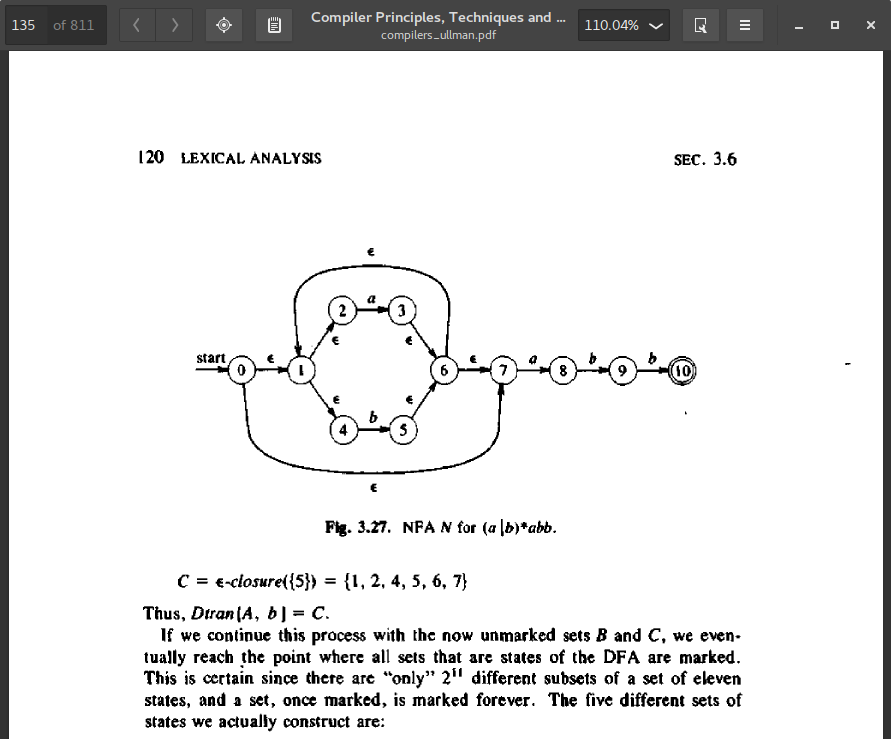
\includegraphics[width=\textwidth]{AFN.png}
        \caption{AFN que reconoce el lenguaje $(a|b)^{*}abb$.}
        \label{fig:AFN}
        \end{center}
    \end{figure}

Es por esto que se utiliza el siguiente algoritmo (construcciones de subconjuntos) para pasar de un AFN a un AFD \cite{compis}. Este algoritmo se basa en que cada estado en el AFD es igual a un subconjunto de estados del AFN.

\begin{figure}[H]
        \begin{center}
        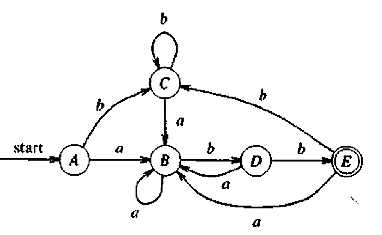
\includegraphics[width=\textwidth]{AFD.png}
        \caption{AFD que reconoce el mismo lenguje que el AFN de la figura \ref{AFN}.}
        \label{fig:AFD}
        \end{center}
    \end{figure}

\section{Desarrollo}
\section{Resultados}
    \begin{figure}[H]
        \begin{center}
        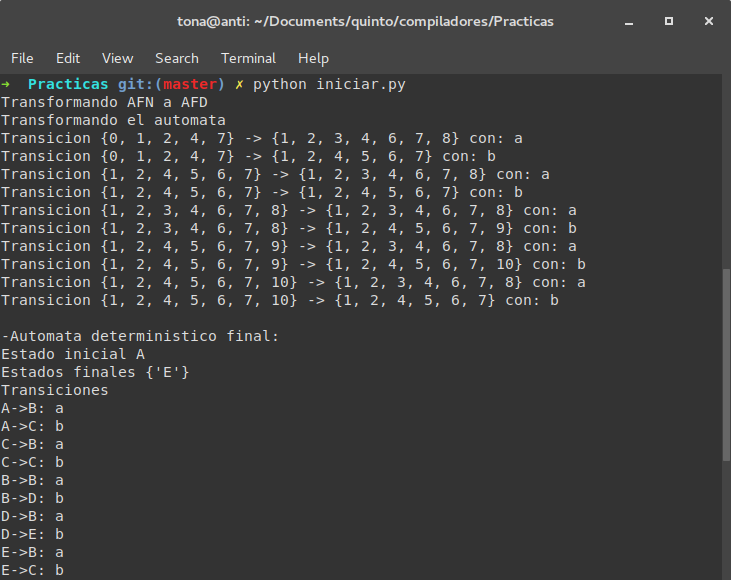
\includegraphics[width=\textwidth]{1.png}
        \caption{Estados como subconjuntos y estados reetiquetados en el automata deterministico final.}
        \label{fig:creacion}
        \end{center}
    \end{figure}
    \begin{figure}[H]
        \begin{center}
        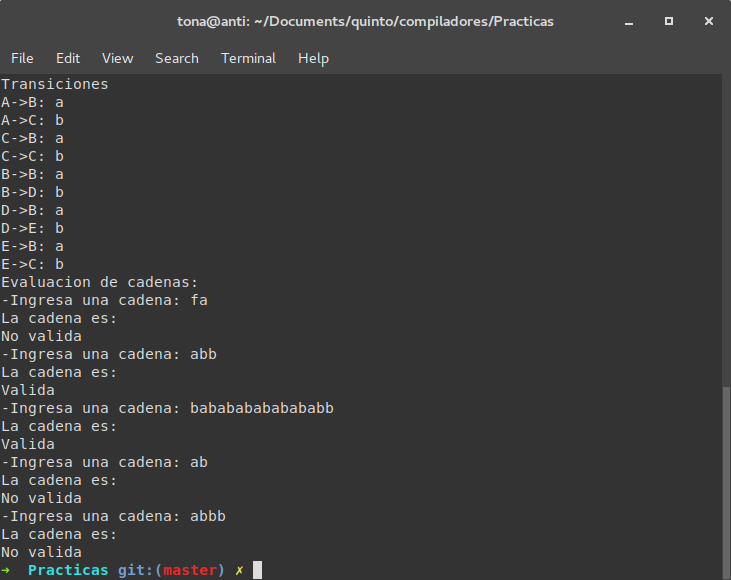
\includegraphics[width=\textwidth]{2.png}
        \caption{Pruebas realizadas sobre el automata que se obtuvo a travez de la transorfación.}
        \label{fig:pruebas}
        \end{center}
    \end{figure}
\section{Conclusiones}
    El desarrollo de esta práctica fue sencillo debido a que al tener los algoritmos ya definidos \cite{compis} solo se tuvo que modelar dichos algoritmos en un lenguaje orientado a objetos en este caso Python y después combinar esta práctica con la primer práctica realizada para la evaluación de cadenas. 
    
    Además, la realización de esta practica y las anteriores permitio entender la importancia que tienen las expresiones regulares y los automatas en el analisis lexico de un compilador. Es por esto que para este punto la elaboración de un analizador lexico personal es posible.
    \bibliography{bibliografia} 
    \bibliographystyle{ieeetr}
\end{document}
